% !TEX root = ../main.tex

% = = = = = = = = = = = = = = = = = = = = = = = = = = = = = = = = = = = = = = = = = =

\section{Introductory Remarks}



\section{Classification}

\subsection{Retail Changes}
This is not a standardized pattern. The development team must consider the ways to upgrade the contracts before deploying the smart contract. Known patterns are different on the level of intervention to change the logic that they need in the future. We will describe three famous patterns here:

\paragraph{Parameter Configuration}. The easiest way to upgrade the logic of the smart contract is to have some critical parameter that can change the whole logic of the system and then have a setter function to change these parameters if the system needs upgrades. The best example for this type of upgradeability is MakeDao project. In Maker there are some variables like Dai Saving Rate (DSR) or Stability fee that can be changed through governance vote. The logic behind the smart contract and the economics of the Dapp completely depends on these variables.

\paragraph{Strategy pattern}. The strategy pattern is an easy way for changing part of the code in a contract responsible for a specific feature. Instead of implementing a function in your contract to take care of a specific task, you call into a separate contract to take care of that – and by switching implementations of that contract, you can switch between different strategies.
An example for this pattern is Compound project and how they used strategy pattern for their interest rate model. There is a interest rate model contract in Compound that can be changed during the time. 

\paragraph{Pluggable Modules}. In this pattern we have a core contract that have some immutable features and have the ability to register new modules and features to the main contract. This pattern is mostly used in wallets and DeFi services like DeFi saver and InstaDapp. Users can decide to add new features into their wallet. 

\subsection{Wholesale Changes}

\subsubsection{Contract Migration}

In the migration plan we should write a new contract with our desired new logic. The challenge here is to 
\begin{enumerate}
    \item Grab the needed data (from previous contract or new data): 
    It depends on the data type. It is easy for simple data structures (\eg uint, address, or even arrays) to collect the data just by reading storage slots from the 0 slot. we should take care of complex structures (\eg mapping) in the latest versions of our contract by adding event updates whenever a data added to a mapping variable. In case of an upgrade we can use Logs to find storage slot (using key hash) and collect the data.
    Sometime we need to push new data into our upgraded smart contract. For example in airdrops we need new coin to be added to some specific addresses. 
    \item Push the data into the new contract: 
    Using Constructor, we can use batch transfer function with arrays of addresses and amounts as inputs. This way we can push lots of data using a single transaction. One limitation here is block gas limit. If we exceeds the block gas limit we need to push all data in different blocks (pausing in the first block and unpause at the end). Recently, Devs are using merkle distribution tree to push data on to the smart contracts.
    The most important thing here is the cost of pushing data to the new version. It depends on 1)the number of storage slots to be updated and 2)Method used to push the data on-chain. (Can be tested). 
  \end{enumerate}

Contract Migration is less riskier than other types of upgrades, not cost effective compare to some upgradability types but more decentralized to the other solutions. It's not good for frequent updates.The other advantage of this method is that it removes transaction gas cost needed for patterns like proxy, registry or call-based methods.

%https://blog.trailofbits.com/2018/10/29/how-contract-migration-works/
% Migration 300,000 balances = $7500 in october 2018



\subsubsection{Data Separation patterns}
In this type we aim to make logic and storage contracts separate. In case of the upgrade we just need to update the logic contract and link the new version to the storage contract.

Here we have 2 different choices using Call method or Delegate Call method to link storage and logic contracts together.

\paragraph{Call based patterns}

Data separation patterns keeps logic and data in different contracts. The logic contract is the one that can be upgraded. In this pattern user is supposed to call the logic contract and the logic contract will call the storage contract.

There are two concerns in this approach: how to store data and how to perform an upgrade.

\textit{Storage. }The easiest way to store data in storage contract is to have a modifier on the setter functions in the storage contract that allow just the logic contract to change the variables. The owner of the contract can change the address of logic contract for the modifier.
In this approach for adding a new persistent variable, a new data contract should be deployed which may be costly in case that the application needs lots of upgrades.

The other way to store data is so called Eternal storage (ERC930). Eternal storage uses mapping (key-value pair) to store data, using one mapping per type of variable. The EVM storage layout and how it handles mapping helps the Eternal storage pattern to be more amenable to evolution but also more complex.

\textit{Upgrade implementation. } There are three main ways to implement upgrades using data separation pattern. The easiest way is to change the ownership of storage contract into new upgraded logic contract and then \textbf{Pause} the old contract or set its pointer to 0x0 address. The other solution is to forward the calls receive by the old contract into the new logic contract. The last option is to set a proxy contract that just keeps the address of logic contract and call into logic contract.

\textit{Risks. } (From trail of bits blog)
"We have repeatedly seen clients deploy this pattern incorrectly. For example, one client’s implementation achieved the opposite effect, where a feature was impossible to upgrade because some its logic was located in the data contract.

In our experience, developers also find the EternalStorage pattern challenging to apply consistently. We have seen developers storing their values as bytes32, then applying type conversion to retrieve the original values. This increased the complexity of the data model, and the likelihood of subtle flaws. Developers unfamiliar with complex data structures will make mistakes with this pattern."


\paragraph{DelegateCall-based upgrades}
Similar to data separation pattern here we have two contracts, Storage and Logic contract. we may have more than one logic contract. The difference here is that the user is calling storage contract first, so called proxy contract, and this contract DelegateCall to the logic contract(s).
The main difference between delegatecall and call-based approach is that in delegatecall proxy pattern the storage layout of proxy and logic contract should be the same. The difference between storage layouts will result in storage clashes. 
There are three different methods to mitigate the risk of storage crashes:

\textit{Inherited Storage}. 
In this method the proxy contract and all logic contracts are inherited from a storage contract that contains storage variables. Using this method we are confident that the proxy and logic contracts are using the same storage layout and storage clashes will be mitigated.
After deployment if we need new logic contract with new storage variables, we should deploy a new storage contract that inherits the previous storage contract. Then the new logic contract must inherit the new version of the storage contract.

The downside of this approach is that new logic contracts inherit storage contracts that may contain variables that it do not need. Also, we should take care that newer versions of the logic contract and storage contract coupled together correctly.

This method is not efficient because of variables that declared but not used in some logic contracts. On the other hand, each logic contract is coupled with a storage contract and it is hard to take care of this track. 
\textit{Eternal Storage}. 
In this pattern, we defined mappings for all variable types that we need to use in our logic smart contract. For storing mapping variables EVM selects random slots based on the variable's name so we can mitigate the clashes.
The main problem of this type is that the logic contract and all other contracts that are using the storage must use the mapping structure to access the storage variables and use complex syntax whenever they want to access a variable.
Also it is hard to use eternal storage for complex variables like mappings and structure (need mapping of mapping pattern).
It is hard to find the state variable of the proxy smart contract because we store them in arbitrary slots of the storage. we cannot add new state variables using this method.
\textit{Unstructured Storage}. 
The other way of mitigating the storage clash is to assign some randomly selected slots to critical variables like address of logic contract. For instance, open zeppling uses hash of "org.zeppelinos.proxy.implementation" to store the address of the logic contract in this slot.

The downside of this approach is that we need getter and setter function for each variable. We also can use unstructured storage for simple variables and not for mapping and structures.

\begin{figure}
  \centering
    
      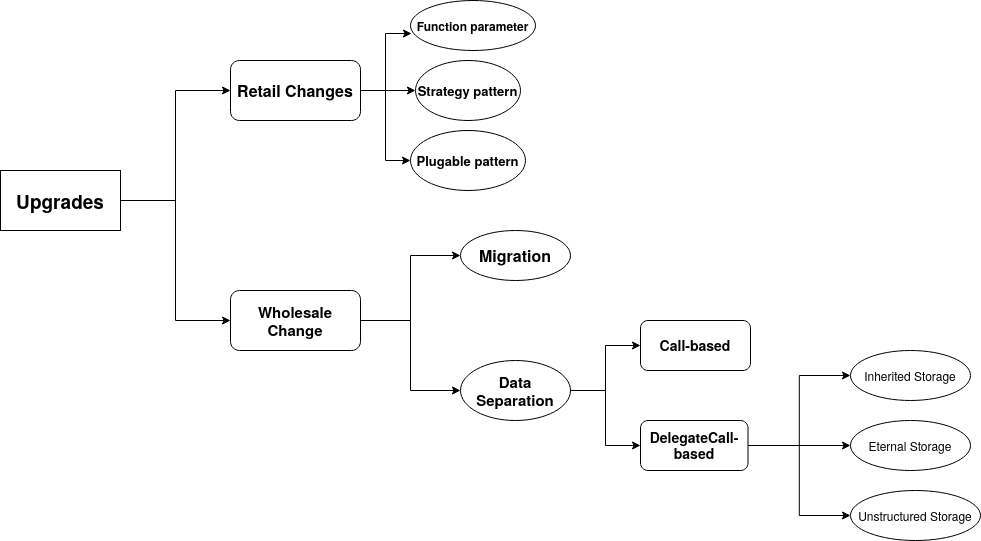
\includegraphics[width=0.9\textwidth]{figures/Chart.png}
  \caption{Classification}
 \end{figure}
% \begin{figure}
%   \includegraphics[width=\textwidth]{fig1.eps}
%   \caption{A figure caption is always placed below the illustration.
%   Please note that short captions are centered, while long ones are
%   justified by the macro package automatically.} \label{fig1}
%   \end{figure}
% \section{Concluding Remarks}


% \subsection{Registry pattern}
% Registry contracts are probably the simplest approach to upgradeability. Registry pattern consist of two main contracts: registry and logic contract. Registry contract holds the addresses of logic contracts and whenever it receives a transaction it will pass it to the related logic contract. 
% If the development team decide to upgrade the smart contract, they can deploy another smart contract and then just change the pointer of the registry smart contact to the new smart contract.

% The main disadvantage of this approach is that in upgrading event, there should be a manual or automated migration plan to transfer data from the old contract into the new upgrade smart contract.
% Another drawback of this pattern is that it also introduces additional complexity for external clients who would also need to call into the registry before interacting with the system


%Idea: see how frequent each project uses its upgradeability feature to upgrade the contract and why?

%In proxy storage layout you should take care that: 
% 1. never remove variable
% 2. never change var type
% 3. never change inheritance order


%Implementation of Eternal storage in call based upgrades: https://medium.com/cardstack/upgradable-contracts-in-solidity-d5af87f0f913
% Good classificaton: https://medium.com/1milliondevs/solidity-storage-layout-for-proxy-contracts-and-diamonds-c4f009b6903
% New storage type *Dimond Storage*: https://medium.com/1milliondevs/new-storage-layout-for-proxy-contracts-and-diamonds-98d01d0eadb
%https://medium.com/1milliondevs/new-storage-layout-for-proxy-contracts-and-diamonds-98d01d0eadb
% Upgradability checklist: https://blog.trailofbits.com/2020/06/12/upgradeable-contracts-made-safer-with-crytic/



%ToDo: Write about OpenZeppling upgrade bug : https://blog.trailofbits.com/2018/09/05/contract-upgrade-anti-patterns/
%ToDo: Gas cost comparison between different implementation (using different number and types of the storage variables)